\normaltrue \difficilefalse \tdifficilefalse
\correctionfalse

%\UPSTIidClasse{11} % 11 sup, 12 spé
%\newcommand{\UPSTIidClasse}{11}

\exer{La Seine Musicale$\star$ \label{B2:07:39}}
\setcounter{numques}{0}
\UPSTIcompetence[2]{B2-07}
\index{Compétence B2-07}
\index{La Seine Musicale}
\ifcorrection
\else
\textbf{Pas de corrigé pour cet exercice.}
\fi

\ifprof
\else
Soit le schéma-blocs suivant. 
\begin{figure}[H]
\centering
\rotatebox{90}{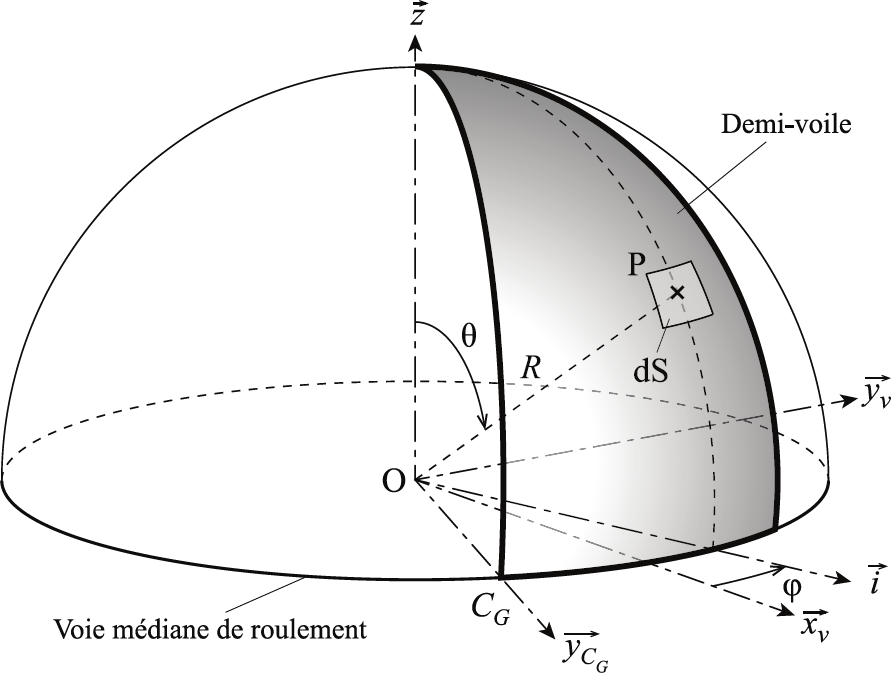
\includegraphics[width=.7\textheight]{39_01}}
%\caption{ \label{fig_39_01}}
\end{figure}
\fi

\question{En considérant que la perturbation $C_{\text{pert}}(p)$ est nulle, déterminer $H_f(p)=\dfrac{\Omega_m(p)}{\Omega_c(p)}$ sous forme canonique.}
\ifprof
\else
\fi

\question{Exprimer la fonction de transfert $H_r(p)=\dfrac{\Omega_m(p)}{C_{\text{pert}}(p)}$ en la mettant sous la forme : $H_r(p)=-\dfrac{\alpha \left(1+\tau p\right)}{1+\gamma p+\delta p^2}$. Exprimer $\alpha$, $\tau$, $\gamma$ et $\delta$ en fonction des différents paramètres de l’étude.}
\ifprof ~\\
\else
\fi

\question{Exprimer $X_{\text{ch}}(p)$ en fonction de $\Omega_m(p)$ et $C_{\text{pert}}(p)$.}
\ifprof ~\\
\else
\fi



\ifprof
\else
\begin{flushright}
\footnotesize{Corrigé  voir \ref{B2:07:39}.}
\end{flushright}%
\fi